\documentclass{article}

\usepackage{amsthm}
\usepackage{amsfonts}
\usepackage{amsmath}
\usepackage{amssymb}
\usepackage{fullpage}
\usepackage{graphicx}
\usepackage[usenames]{color}
\usepackage{hyperref}
  \hypersetup{
    colorlinks = true,
    urlcolor = blue,       % color of external links using \href
    linkcolor= blue,       % color of internal links 
    citecolor= blue,       % color of links to bibliography
    filecolor= blue,        % color of file links
    }
    
\usepackage{listings}

\definecolor{dkgreen}{rgb}{0,0.6,0}
\definecolor{gray}{rgb}{0.5,0.5,0.5}
\definecolor{mauve}{rgb}{0.58,0,0.82}

\lstset{frame=tb,
  language=haskell,
  aboveskip=3mm,
  belowskip=3mm,
  showstringspaces=false,
  columns=flexible,
  basicstyle={\small\ttfamily},
  numbers=none,
  numberstyle=\tiny\color{gray},
  keywordstyle=\color{blue},
  commentstyle=\color{dkgreen},
  stringstyle=\color{mauve},
  breaklines=true,
  breakatwhitespace=true,
  tabsize=3
}

\theoremstyle{theorem} 
   \newtheorem{theorem}{Theorem}[section]
   \newtheorem{corollary}[theorem]{Corollary}
   \newtheorem{lemma}[theorem]{Lemma}
   \newtheorem{proposition}[theorem]{Proposition}
\theoremstyle{definition}
   \newtheorem{definition}[theorem]{Definition}
   \newtheorem{example}[theorem]{Example}
\theoremstyle{remark}    
  \newtheorem{remark}[theorem]{Remark}


\title{CPSC-402 Report\\Compiler Construction}
\author{Anthony Walujono \\ Chapman University}

\date{\today}

\begin{document}

\maketitle

\begin{abstract}
Short  summary of purpose and content.  
\end{abstract}

\tableofcontents

\section{Introduction}\label{intro}

This will cover everything in Compile Construction.

\section{Homework}\label{homework}
\subsection{Week 1: Searching for Strings}
2.24: Give DFA's accepting the the following languages over the alphabet \{0,1\}:
\newline \indent b) The set of all strings with three consecutive 0's (not necessarily at the end).
\medskip\begin{center}
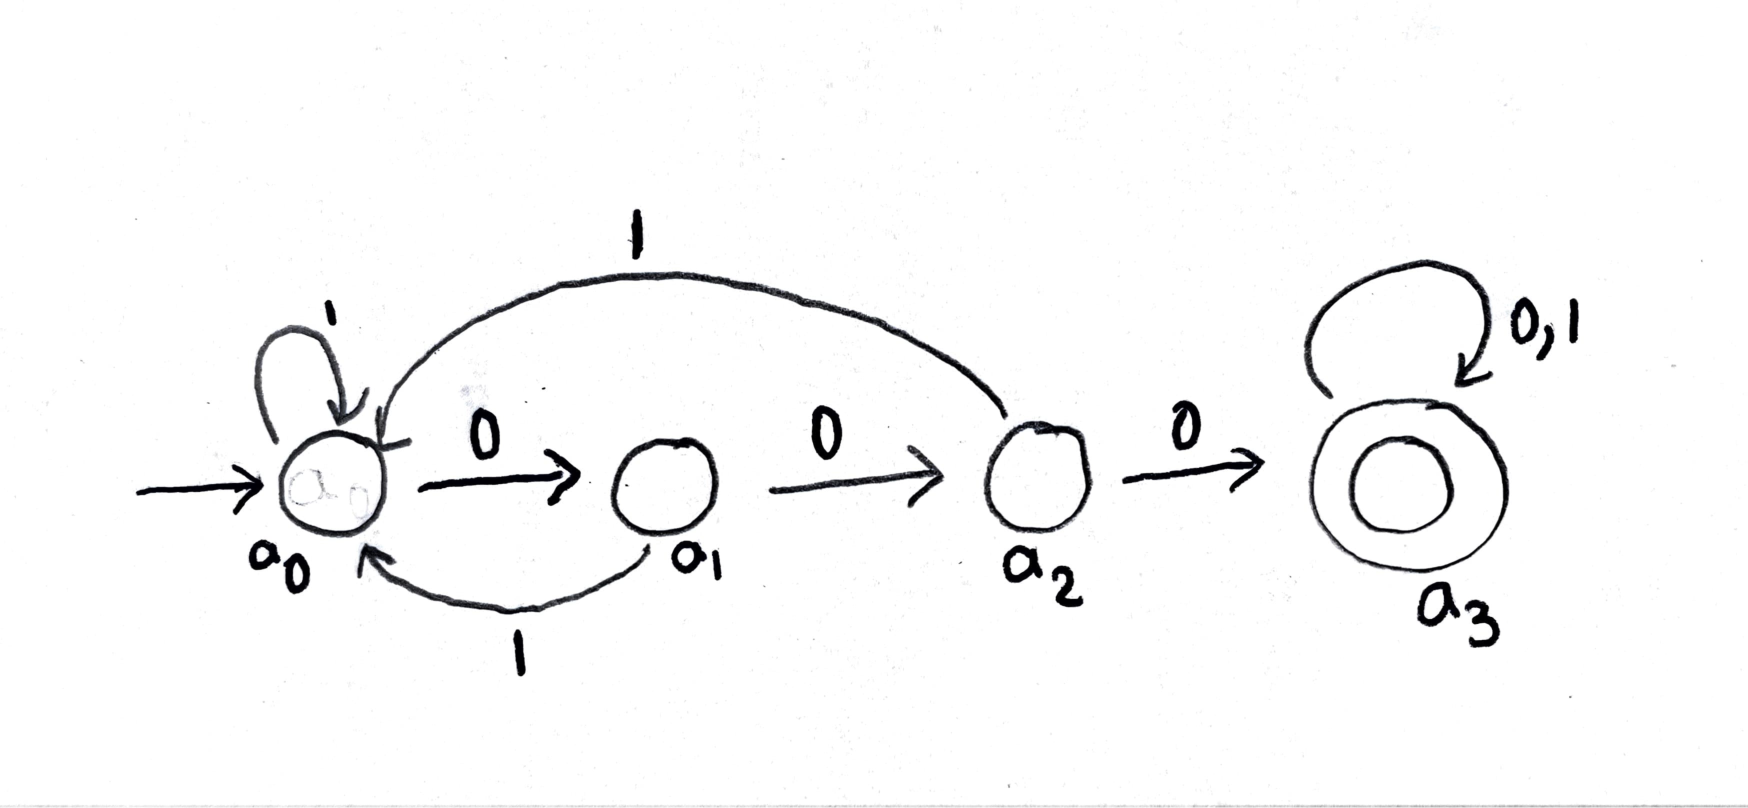
\includegraphics[width=10cm, height=5cm]{Week1b.pdf}
\end{center}
\indent c) The set of strings with 011 as a substring.
\medskip\begin{center}
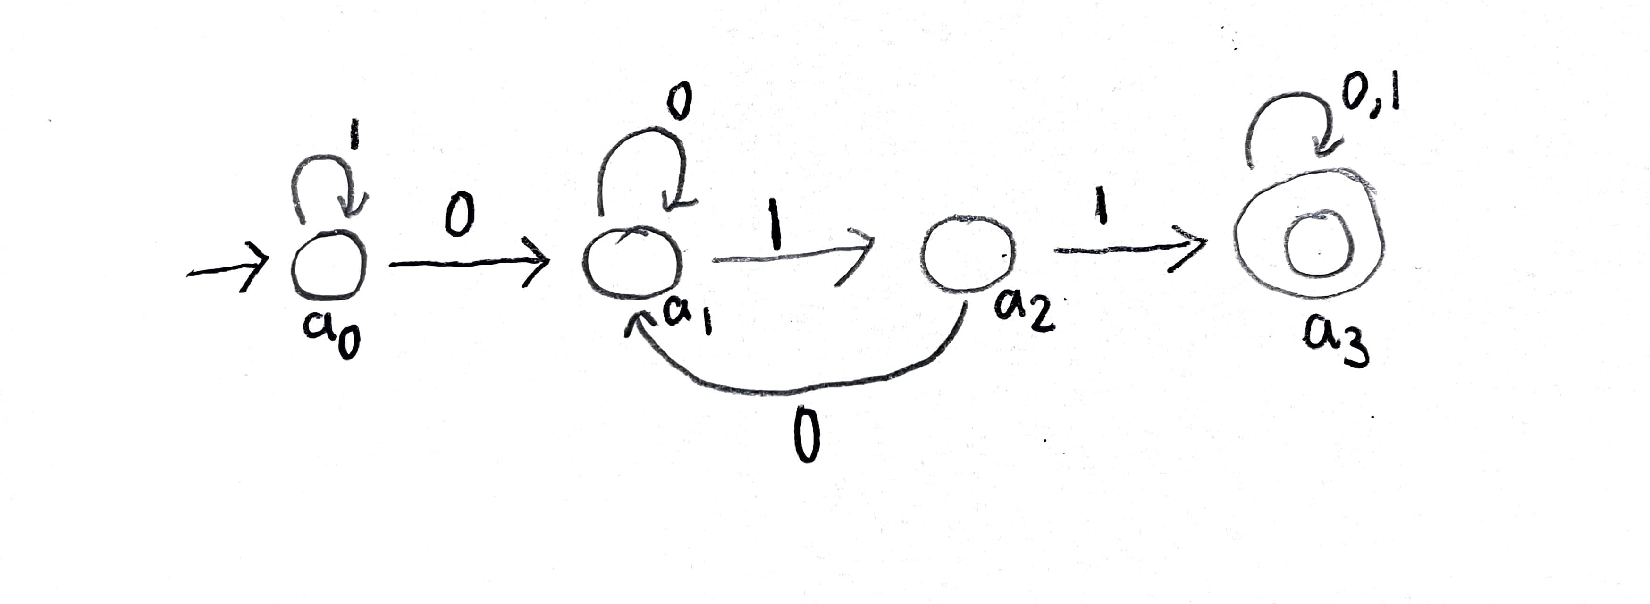
\includegraphics[width=10cm, height=5cm]{Week1c.pdf}
\end{center}

\subsection{Week 2: Regular Expression and NFA}
2.3.4: Give nondeterministic finite automata to accept the following languages. Try to take advantage of nondeterminism as much as possible. 
\medskip\begin{center}
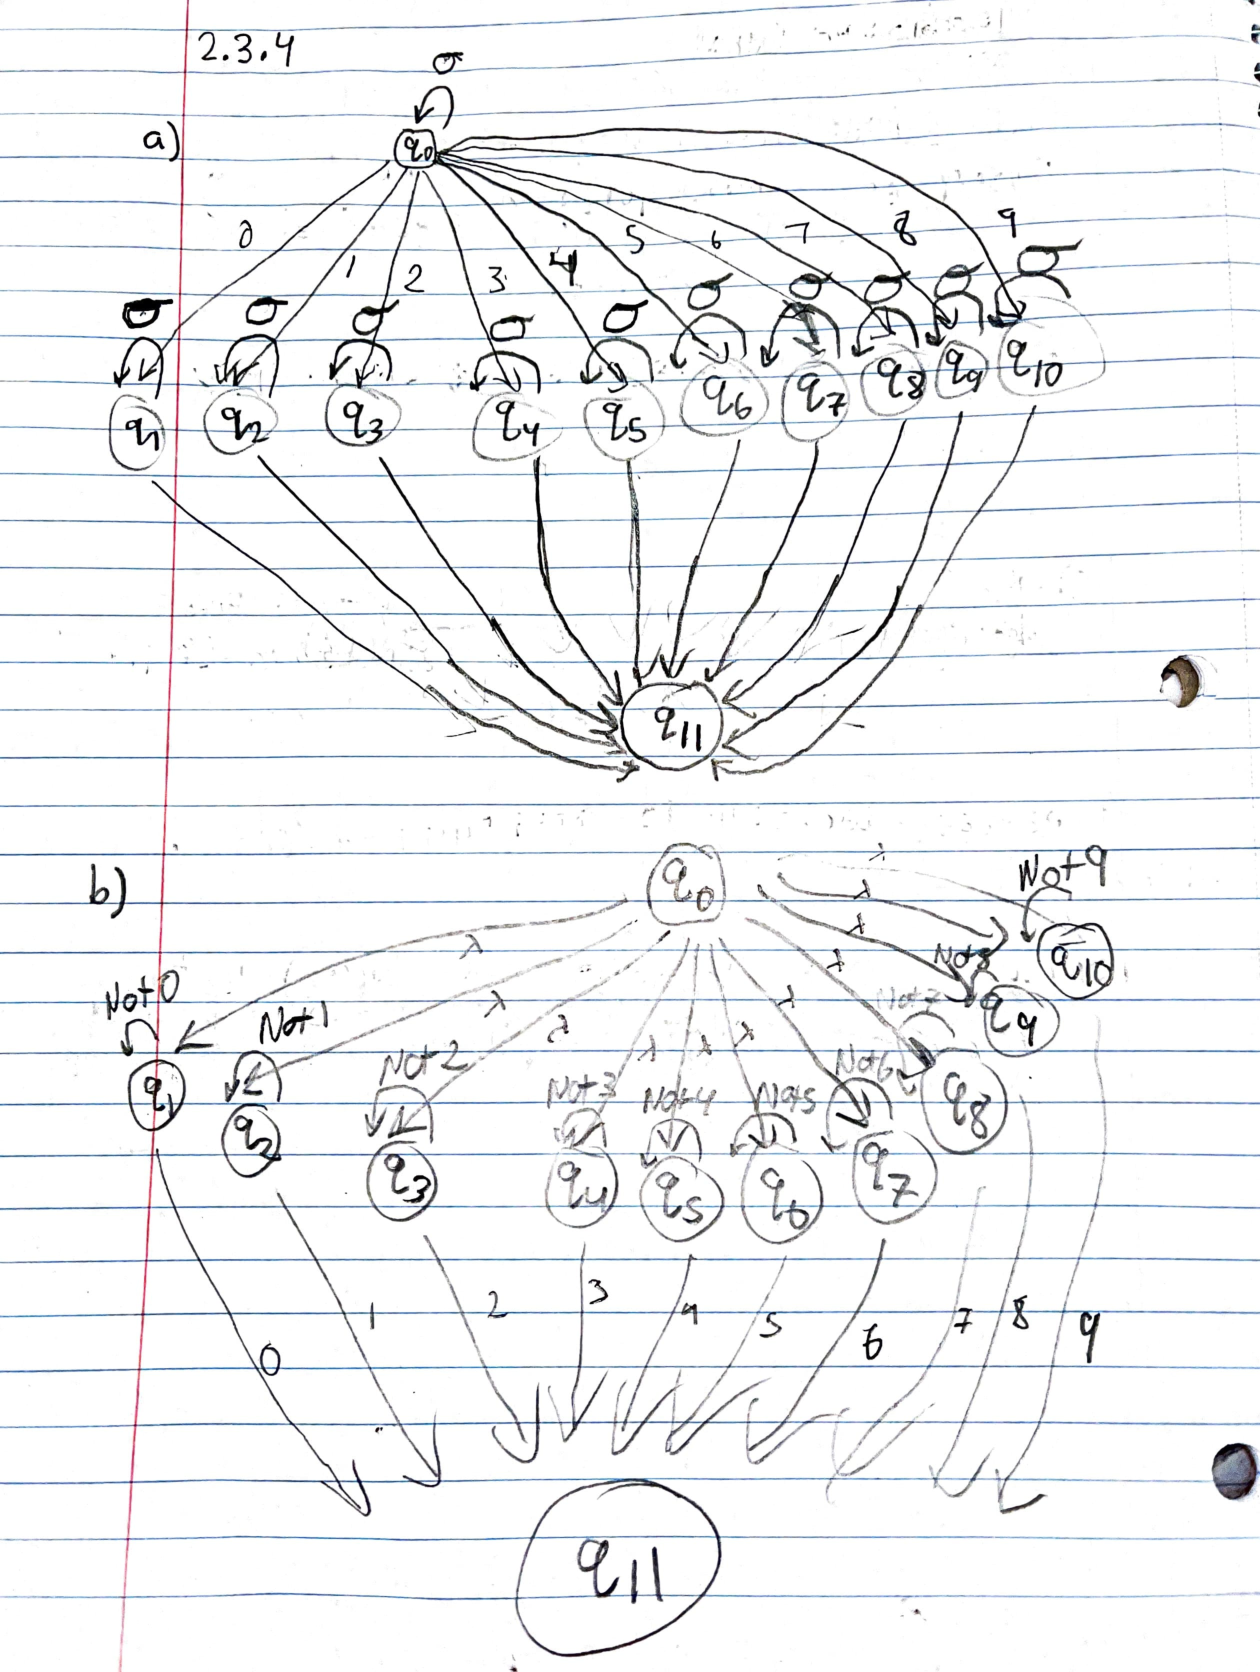
\includegraphics[width=10cm, height=15cm]{Week2_2.3.4ab.pdf}
\end{center}

\medskip\begin{center}
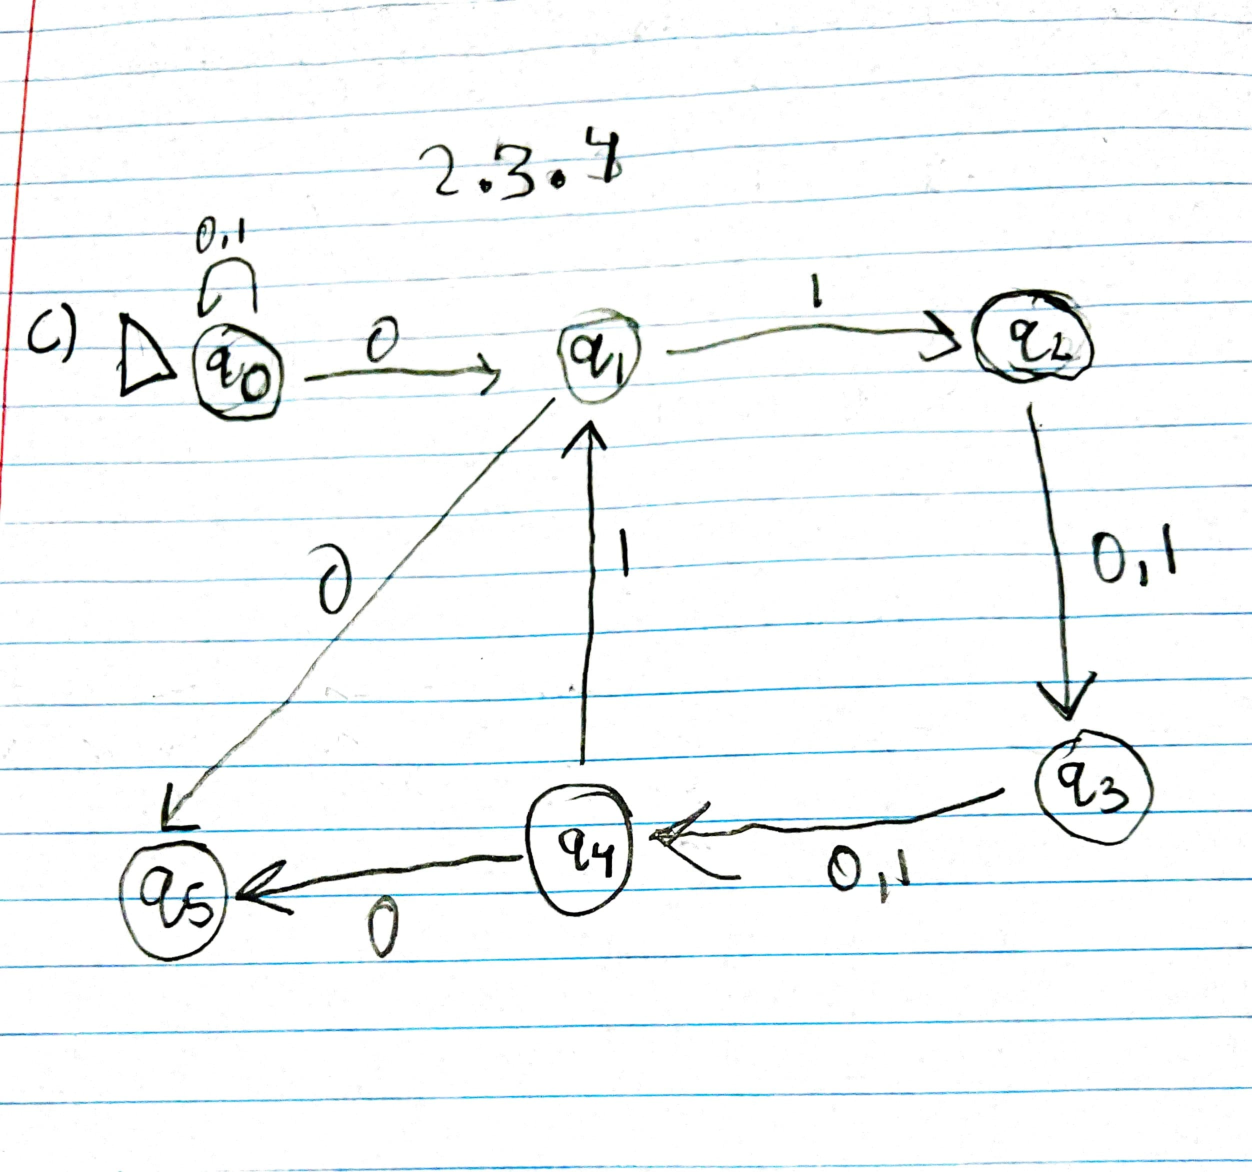
\includegraphics[width=10cm, height=10cm]{Week2_2.3.4c.pdf}
\end{center}

2.5.3: Design  $\epsilon$-NFA's for the following languages. Try to use $\epsilon$ transitions to simplify your design. 
\medskip\begin{center}
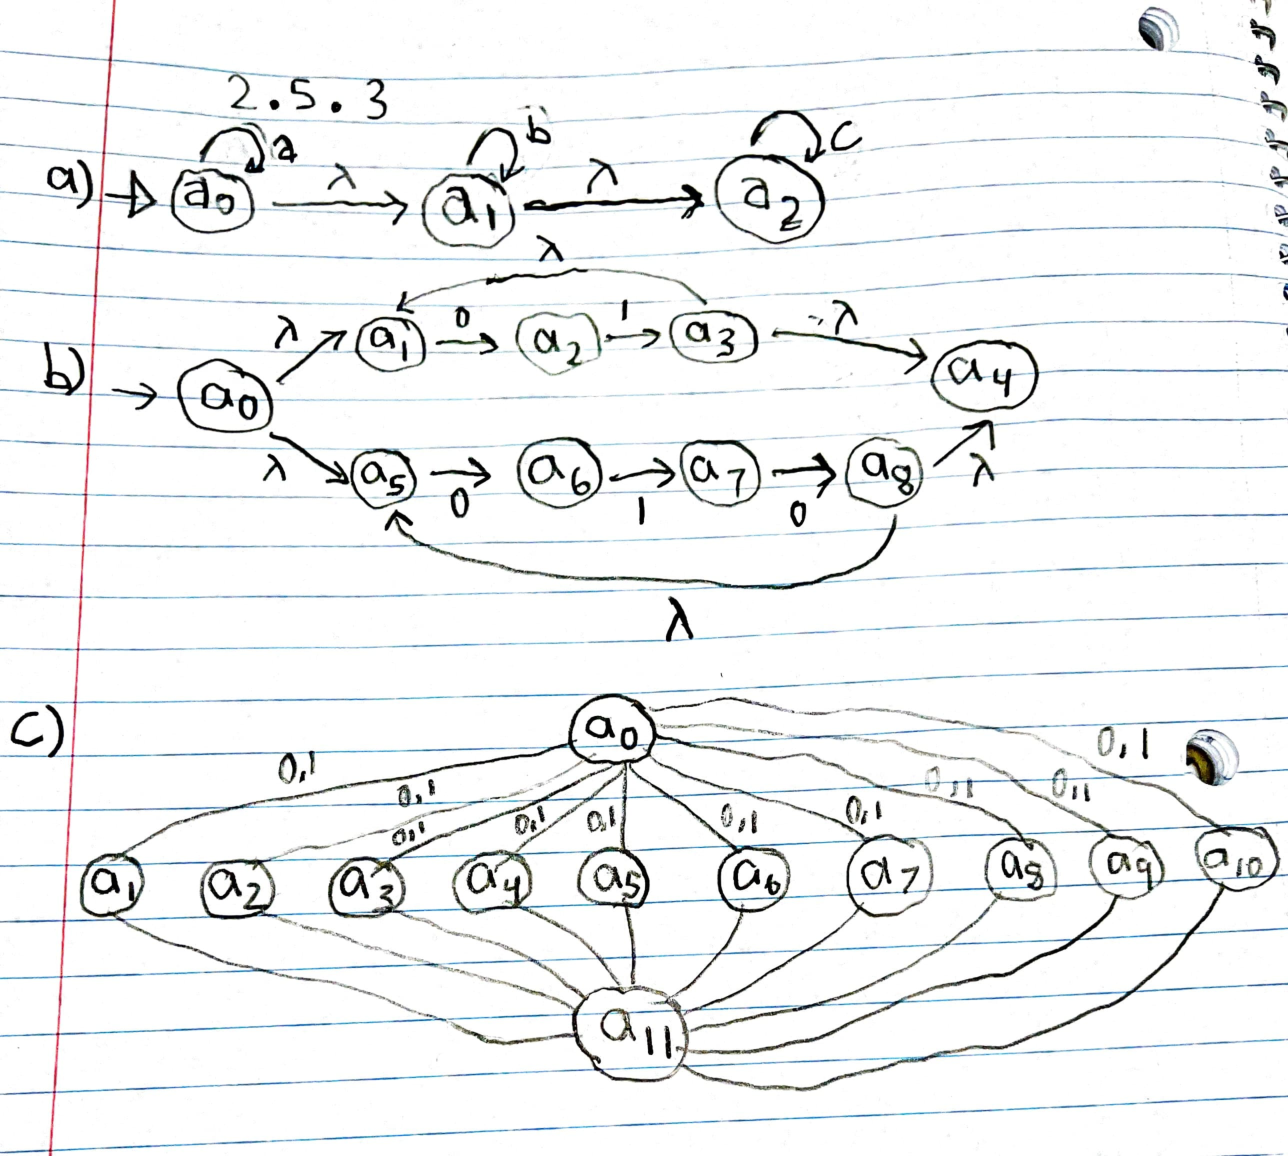
\includegraphics[width=10cm, height=10cm]{Week2_2.5.3.pdf}
\end{center}


\subsection{Week 3: Convert NFAs to DFAs by Hand}
2.3.1: Convert to a DFA the following NFA
\medskip\begin{center}
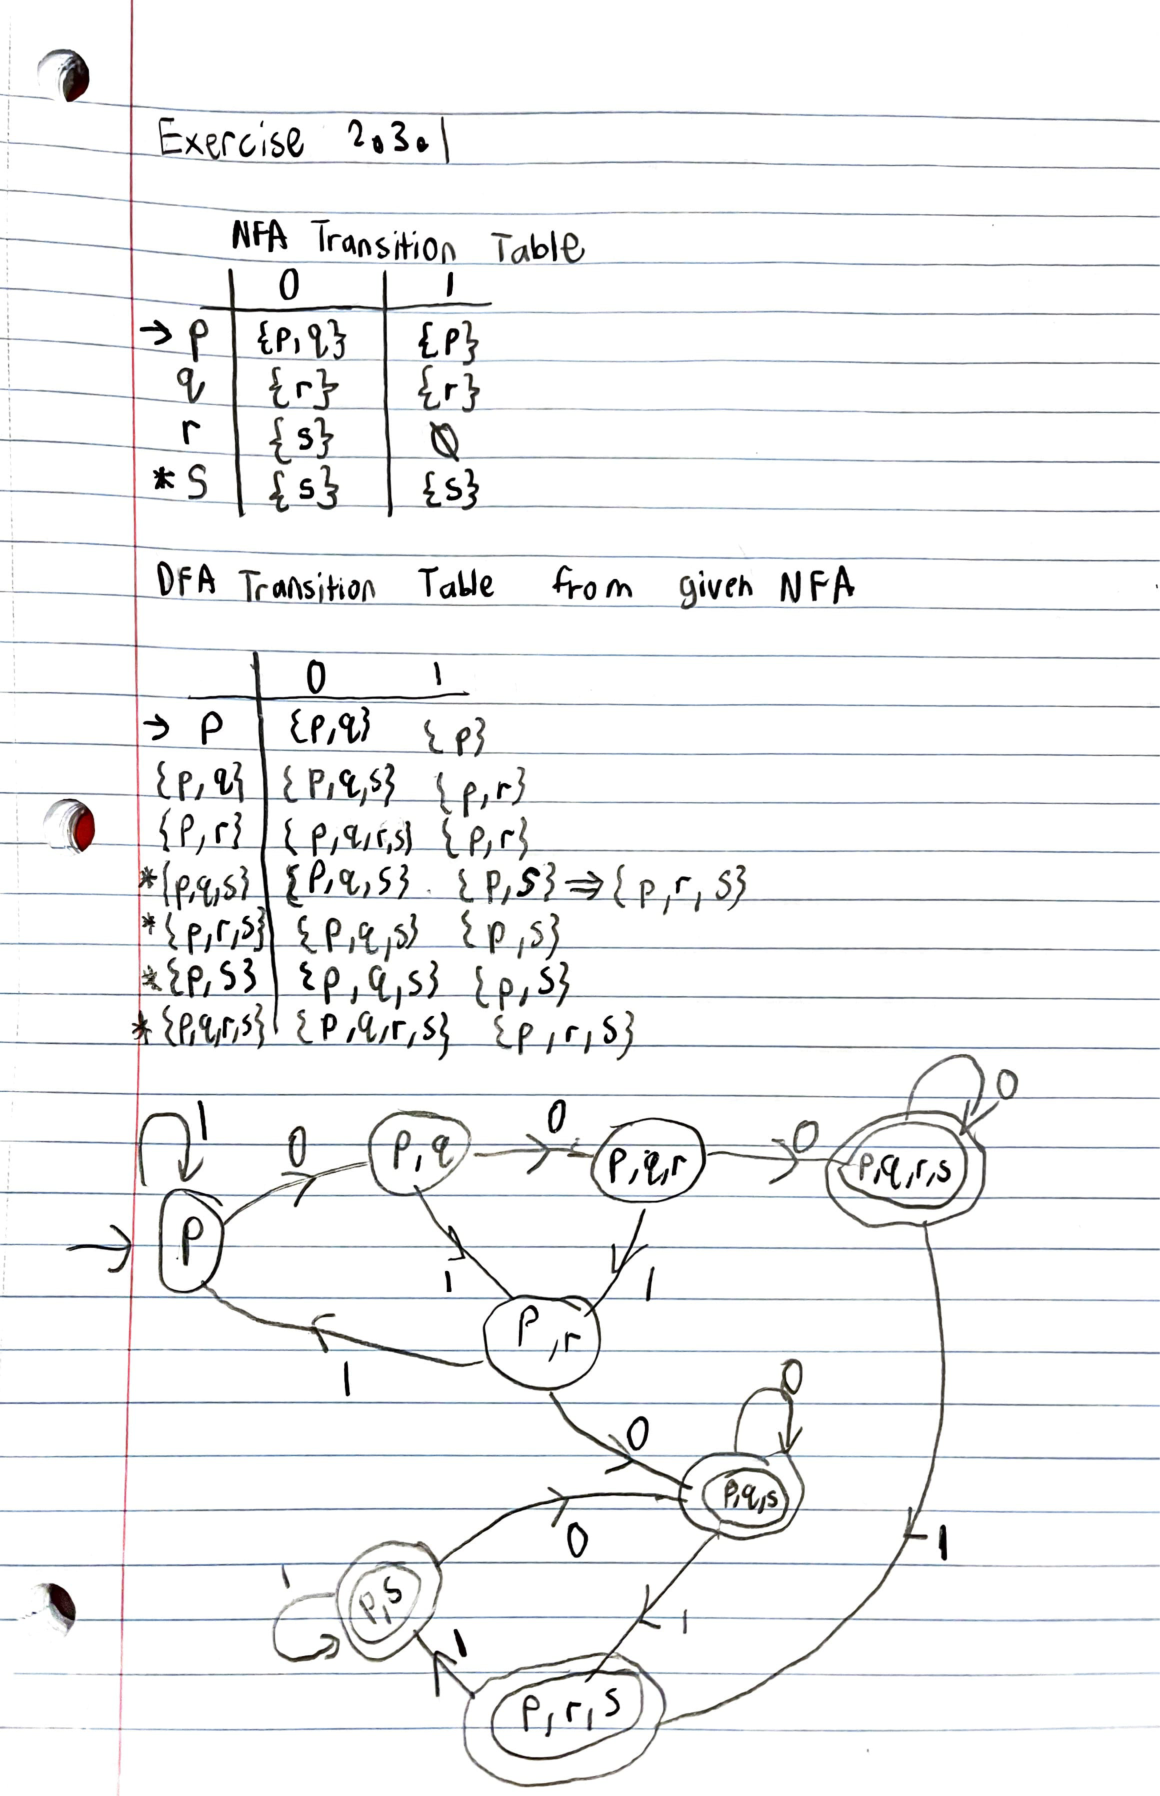
\includegraphics[width=10cm, height=15cm]{Week3_2.3.1.pdf}
\end{center}
2.3.2: Convert to a DFA the following NFA
\medskip\begin{center}
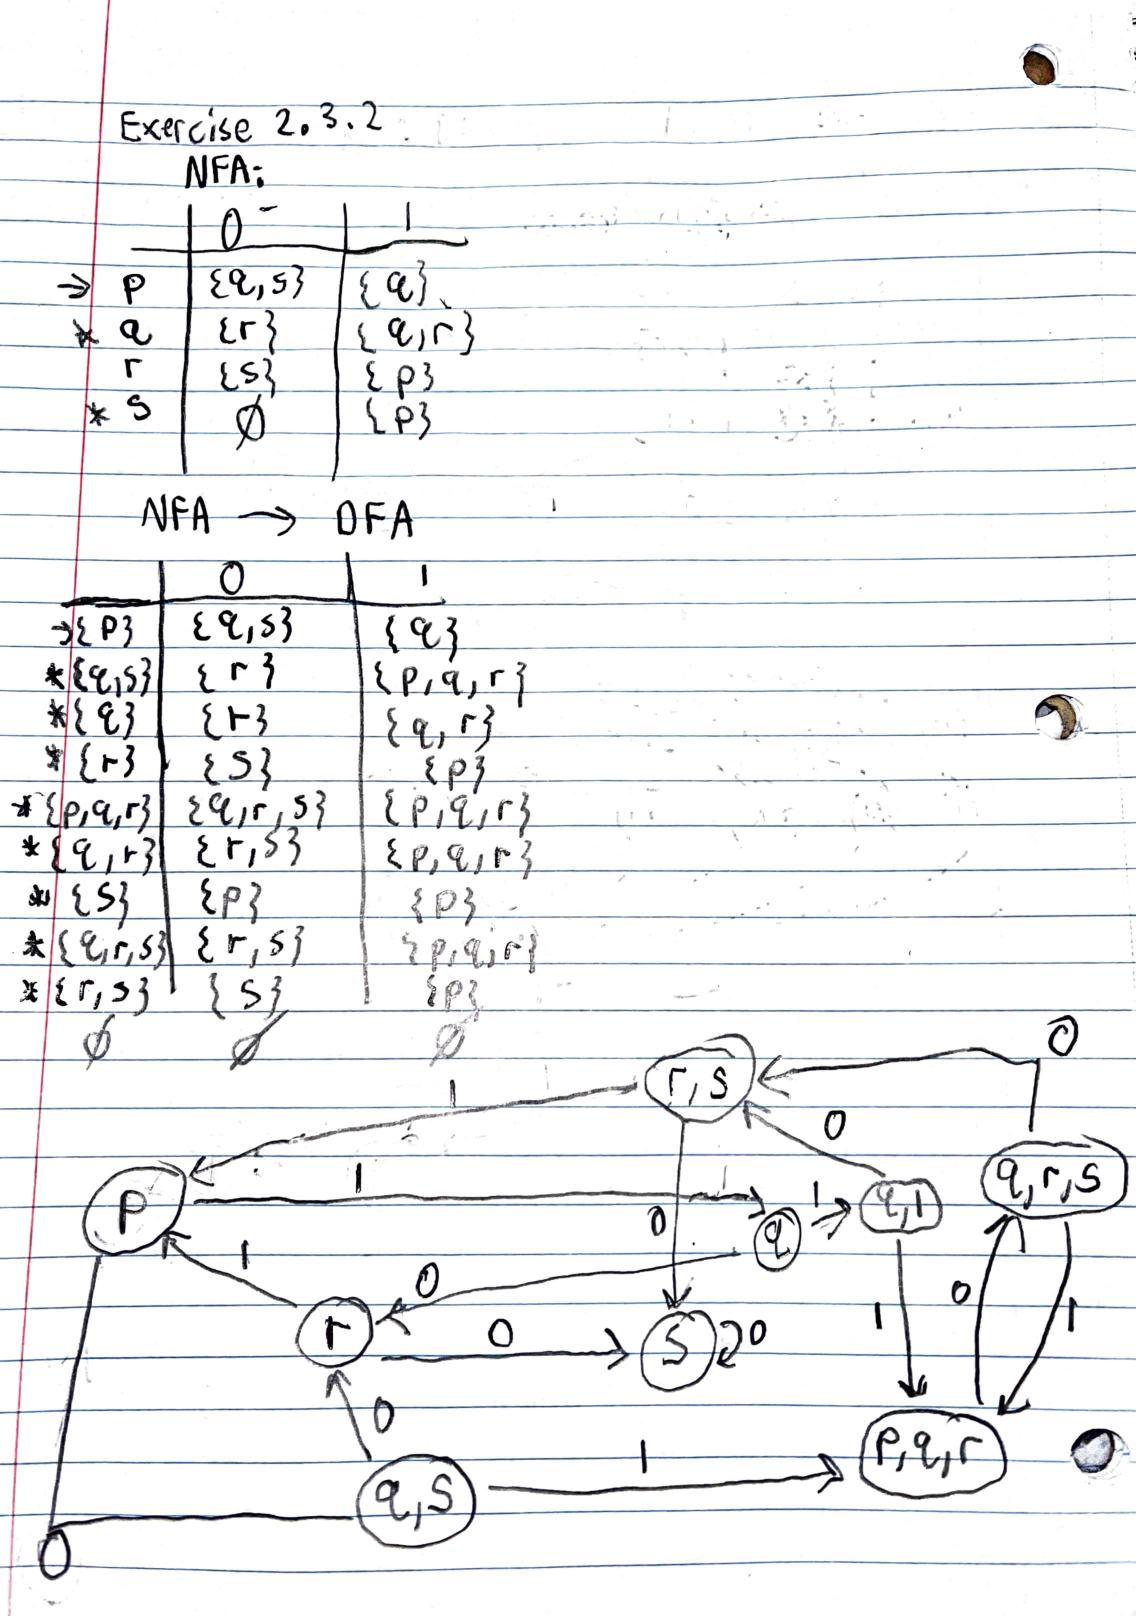
\includegraphics[width=10cm, height=15cm]{Week3_2.3.2.pdf}
\end{center}


\subsection{Week 4: Introduction to Parsing}
Question 1: Write out the parse tree (=concrete syntax tree) for the complete fibonacci program. Think about a question on this for the lecture.
\medskip\begin{center}
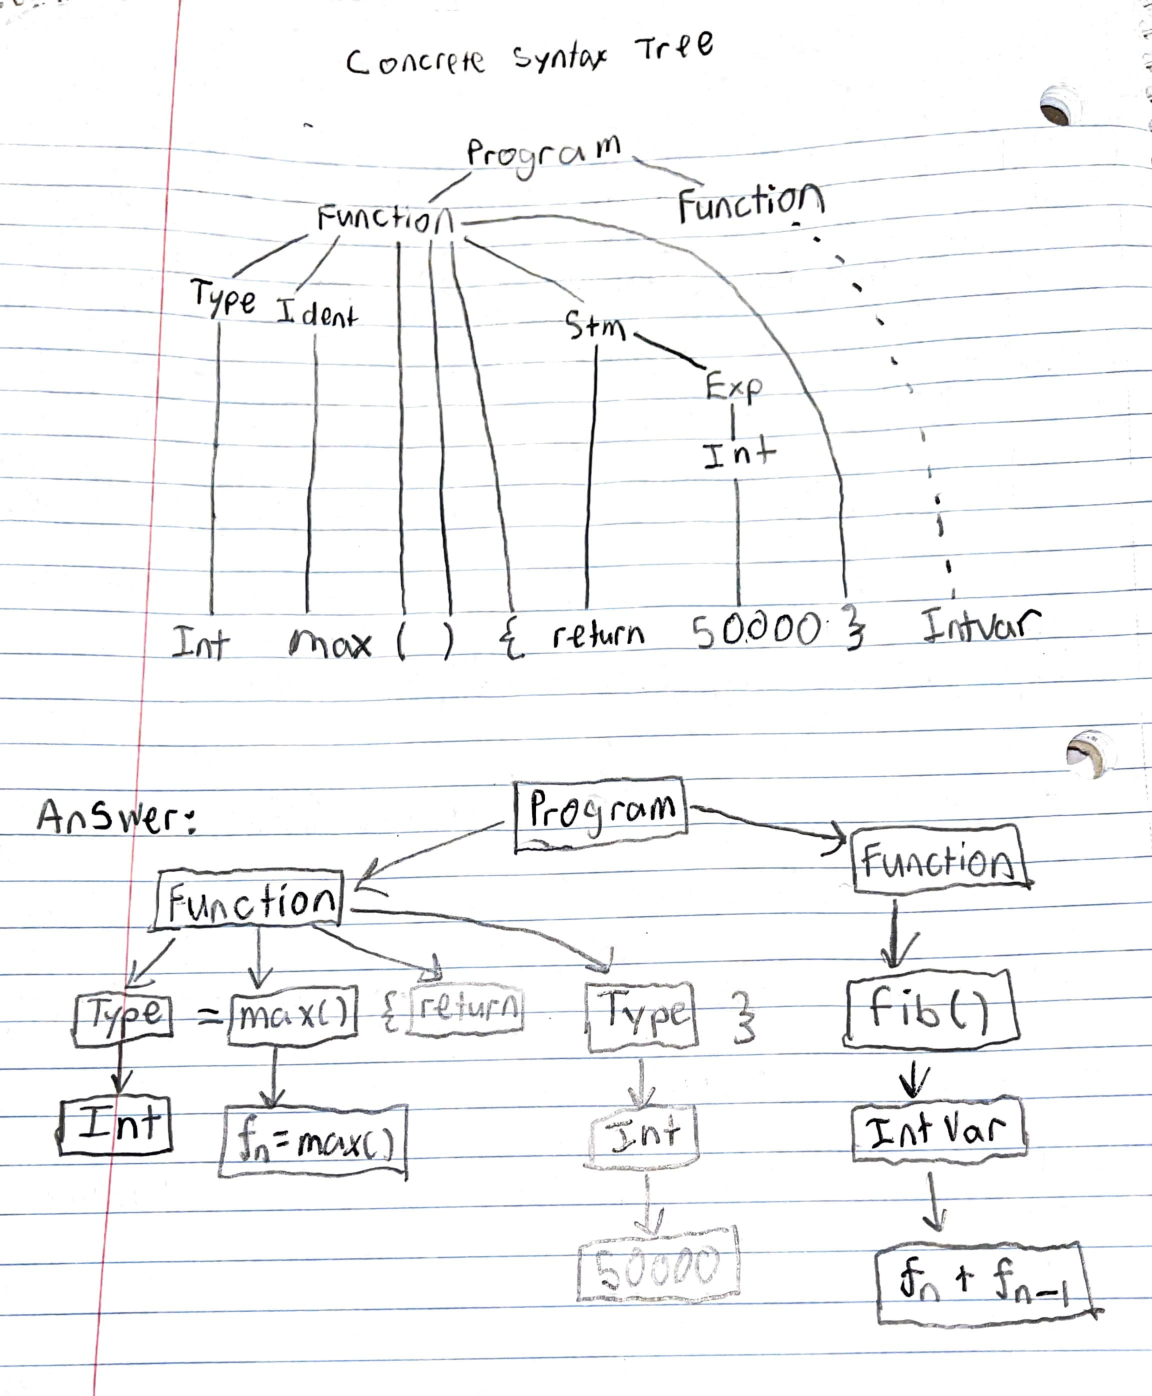
\includegraphics[width=10cm, height=15cm]{Week4Q1.pdf}
\end{center}
Question 2: Write out the abstract syntax tree for the complete fibonacci program. 
\medskip\begin{center}
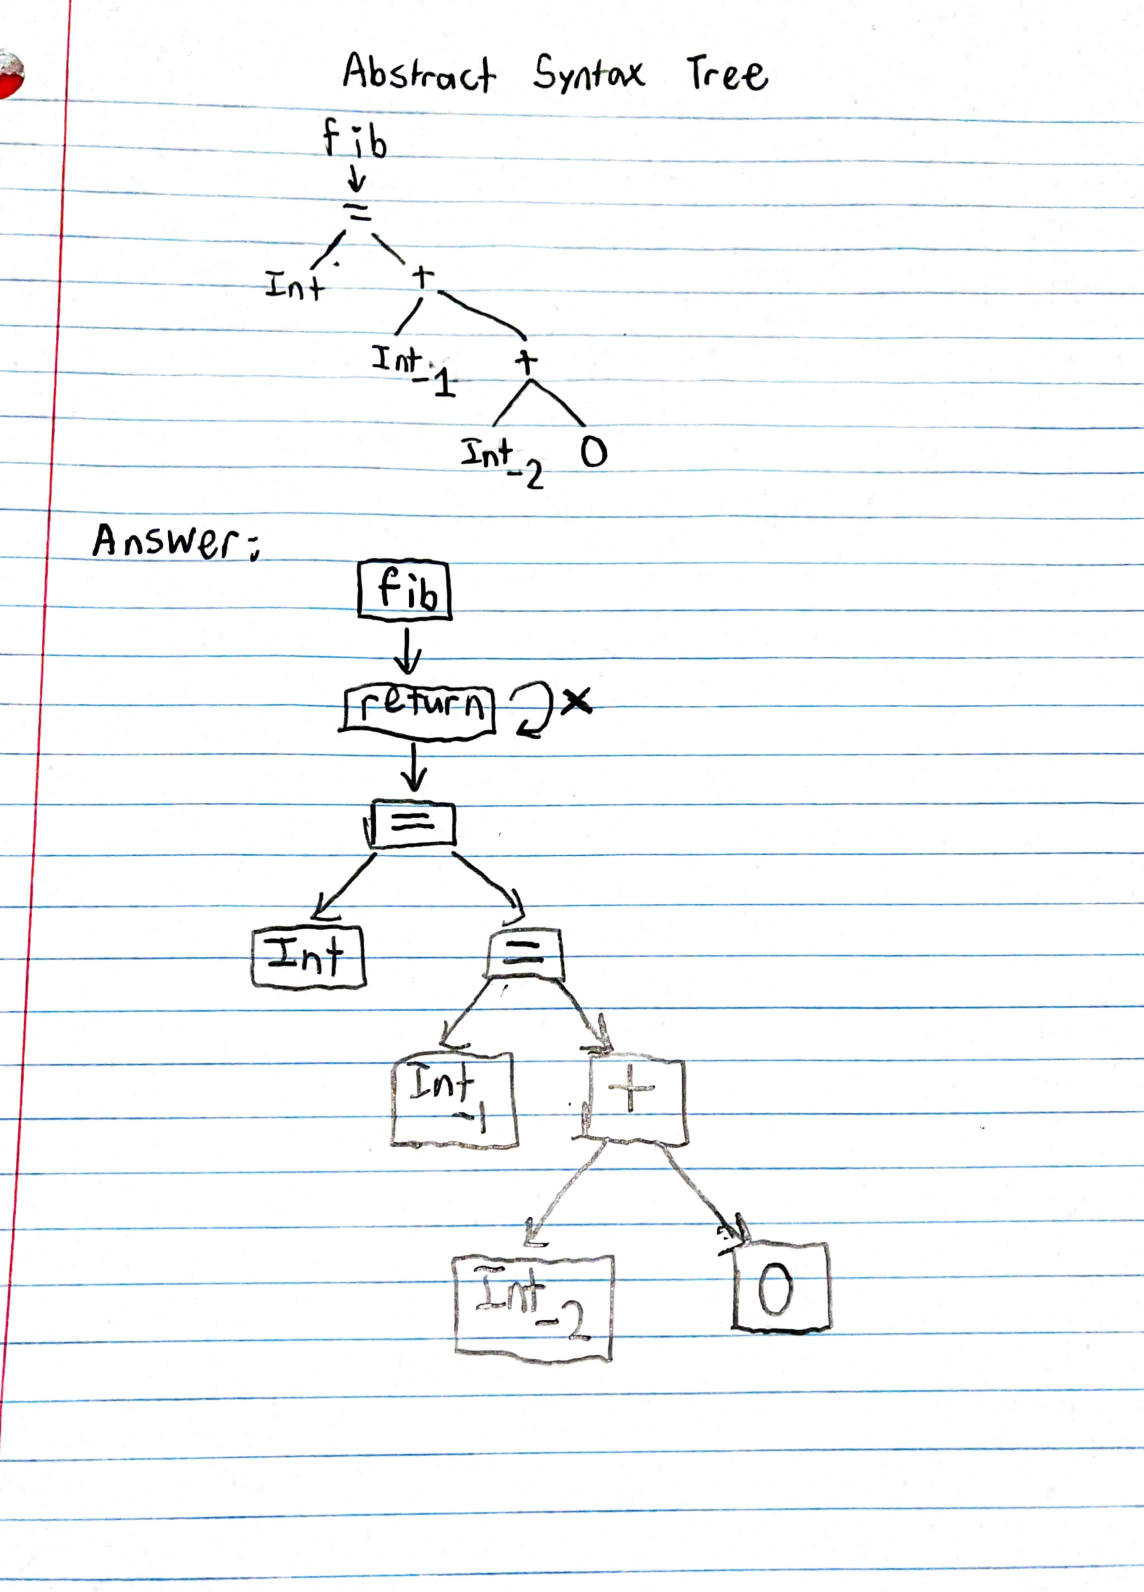
\includegraphics[width=10cm, height=15cm]{Week4Q2.pdf}
\end{center}

\subsection{Week 10: Proof Trees}
\medskip\begin{center}
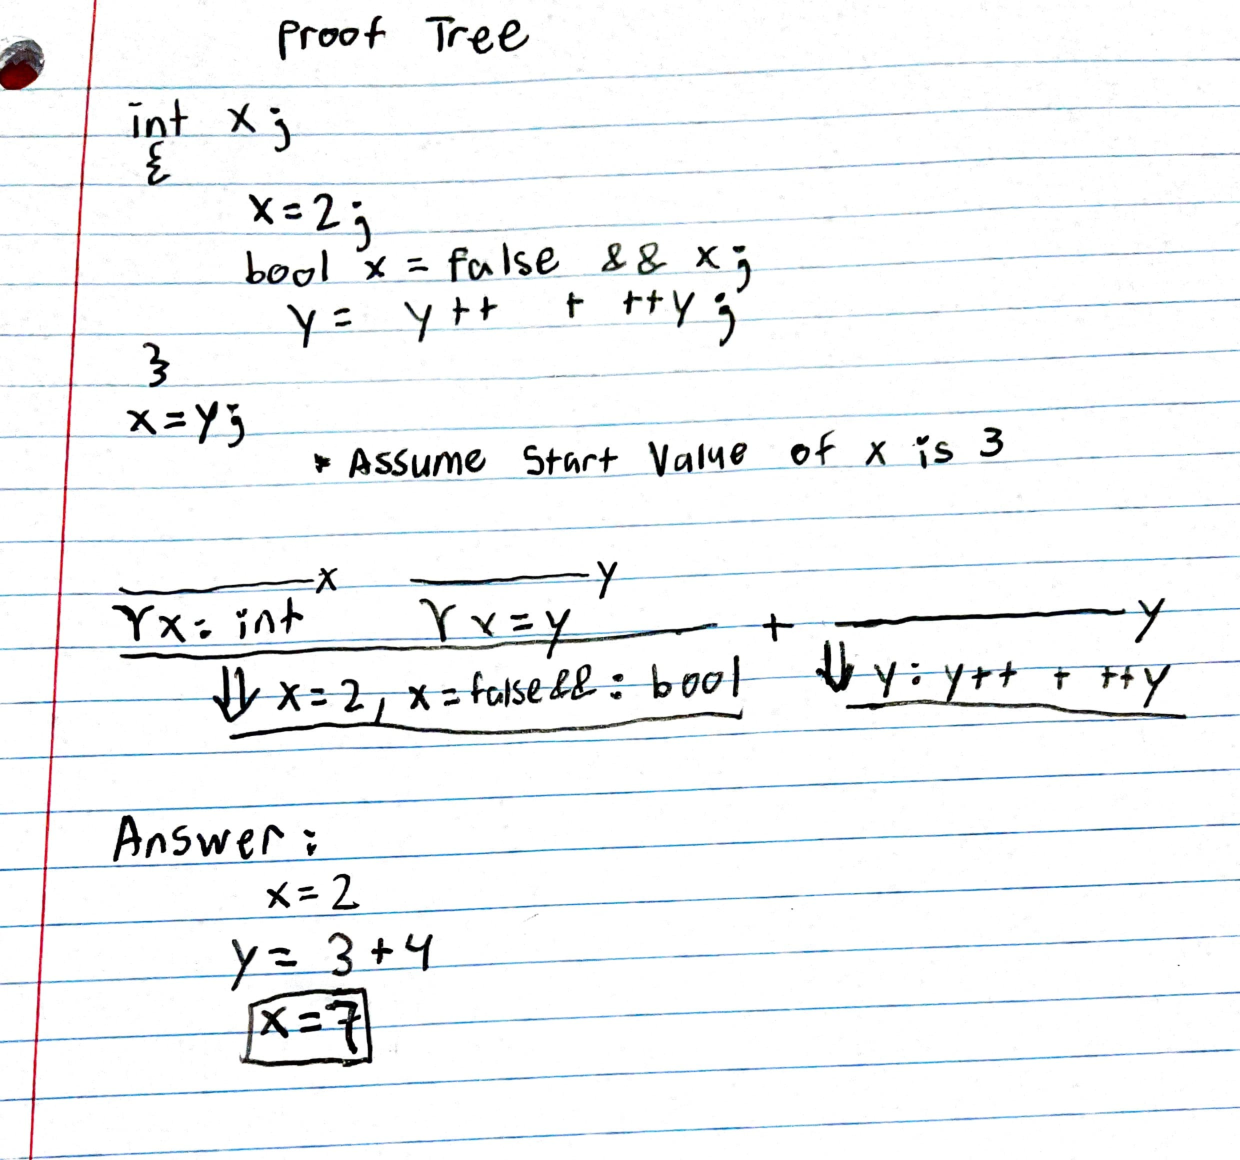
\includegraphics[width=10cm, height=15cm]{Week10.pdf}
\end{center}

\section{Project}
For this project, I plan to explain a compiler. The language that I would use is C++, and the compiler that I would use is g++. A code that I plan to use is recfile.cpp, which is shown below. My target language would be JVM.
\begin{lstlisting}
#include <iostream>
double fahrenheitToCelsius(double fahrenheit){
    double celsius;
 
    celsius = (fahrenheit - 32.0) * 5.0 / 9.0;
    return celsius;
}
 
int main(){
    double fahrenheit;
 
    std::cout << "Enter temperature in fahrenheit (in degrees) ";
    std::cin  >> fahrenheit;
    std::cout << "Temperature in Celsius (in degrees) = "
              << fahrenheitToCelsius(fahrenheit) << std::endl;
}
\end{lstlisting}
Here is  output using x86-64 gcc 12.1
\begin{lstlisting}
fahrenheitToCelsius(double):
        push    rbp
        mov     rbp, rsp
        movsd   QWORD PTR [rbp-24], xmm0
        movsd   xmm0, QWORD PTR [rbp-24]
        movsd   xmm2, QWORD PTR .LC0[rip]
        movapd  xmm1, xmm0
        subsd   xmm1, xmm2
        movsd   xmm0, QWORD PTR .LC1[rip]
        mulsd   xmm0, xmm1
        movsd   xmm1, QWORD PTR .LC2[rip]
        divsd   xmm0, xmm1
        movsd   QWORD PTR [rbp-8], xmm0
        movsd   xmm0, QWORD PTR [rbp-8]
        movq    rax, xmm0
        movq    xmm0, rax
        pop     rbp
        ret
.LC3:
        .string "Enter temperature in fahrenheit (in degrees) "
.LC4:
        .string "Temperature in Celsius (in degrees) = "
main:
        push    rbp
        mov     rbp, rsp
        push    rbx
        sub     rsp, 24
        mov     esi, OFFSET FLAT:.LC3
        mov     edi, OFFSET FLAT:_ZSt4cout
        call    std::basic_ostream<char, std::char_traits<char> >& std::operator<< <std::char_traits<char> >(std::basic_ostream<char, std::char_traits<char> >&, char const*)
        lea     rax, [rbp-24]
        mov     rsi, rax
        mov     edi, OFFSET FLAT:_ZSt3cin
        call    std::basic_istream<char, std::char_traits<char> >::operator>>(double&)
        mov     esi, OFFSET FLAT:.LC4
        mov     edi, OFFSET FLAT:_ZSt4cout
        call    std::basic_ostream<char, std::char_traits<char> >& std::operator<< <std::char_traits<char> >(std::basic_ostream<char, std::char_traits<char> >&, char const*)
        mov     rbx, rax
        mov     rax, QWORD PTR [rbp-24]
        movq    xmm0, rax
        call    fahrenheitToCelsius(double)
        movq    rax, xmm0
        movq    xmm0, rax
        mov     rdi, rbx
        call    std::basic_ostream<char, std::char_traits<char> >::operator<<(double)
        mov     esi, OFFSET FLAT:_ZSt4endlIcSt11char_traitsIcEERSt13basic_ostreamIT_T0_ES6_
        mov     rdi, rax
        call    std::basic_ostream<char, std::char_traits<char> >::operator<<(std::basic_ostream<char, std::char_traits<char> >& (*)(std::basic_ostream<char, std::char_traits<char> >&))
        mov     eax, 0
        mov     rbx, QWORD PTR [rbp-8]
        leave
        ret
__static_initialization_and_destruction_0(int, int):
        push    rbp
        mov     rbp, rsp
        sub     rsp, 16
        mov     DWORD PTR [rbp-4], edi
        mov     DWORD PTR [rbp-8], esi
        cmp     DWORD PTR [rbp-4], 1
        jne     .L7
        cmp     DWORD PTR [rbp-8], 65535
        jne     .L7
        mov     edi, OFFSET FLAT:_ZStL8__ioinit
        call    std::ios_base::Init::Init() [complete object constructor]
        mov     edx, OFFSET FLAT:__dso_handle
        mov     esi, OFFSET FLAT:_ZStL8__ioinit
        mov     edi, OFFSET FLAT:_ZNSt8ios_base4InitD1Ev
        call    __cxa_atexit
.L7:
        nop
        leave
        ret
_GLOBAL__sub_I_fahrenheitToCelsius(double):
        push    rbp
        mov     rbp, rsp
        mov     esi, 65535
        mov     edi, 1
        call    __static_initialization_and_destruction_0(int, int)
        pop     rbp
        ret
.LC0:
        .long   0
        .long   1077936128
.LC1:
        .long   0
        .long   1075052544
.LC2:
        .long   0
        .long   1075970048
\end{lstlisting}
\begin{thebibliography}{99}
\bibitem[HMU]{Hopcroft}
	John E. Hopcroft, Rajeev Motwani, Jeffrey D. Ullman:
\href{http://ce.sharif.edu/courses/94-95/1/ce414-2/resources/root/Text%20Books/Automata/John%20E.%20Hopcroft,%20Rajeev%20Motwani,%20Jeffrey%20D.%20Ullman-Introduction%20to%20Automata%20Theory,%20Languages,%20and%20Computations-Prentice%20Hall%20(2006).pdf}{Introduction to automata theory, languages, and computation,} 3rd Edition. Pearson international edition, Addison-Wesley 2007

\end{thebibliography}

\end{document}